\chapter{The Standard Model and Physics of the Top Quark}
\label{c:the_standard_model_and_top_physics}

\section{The Standard Model}
\label{s:the_standard_model}

The Standard Model is the name given to the theory developed during the course of the 20th century, which
describes the elementary particles that make up all known, observable matter, and the three fundamental forces
they interact by (electromagnetic, weak and strong forces). The Standard Model does not, however, describe the
gravitational force.
% The theory is a combination of the theory of the electroweak interaction and the theory of the strong
% interaction
The Standard Model puts forward twelve fermions, with a spin quantum number of \frac{1}{2}, as the matter
particles, split into two groups of six quarks and six leptons, all of which are split into three generations.
The six quarks are classified according to their charge and flavour: up, down, charm, strange, top and beauty
quarks. The leptons are in turn classified according to their charge and flavour: electron, muon or tau
leptons, together with their corresponding neutrinos). Neutrinos, although originally thought to be massless,
are now believed to carry mass due to the observation of the oscillation of neutrinos between different
flavours. Table~\ref{tab:standard_model} shows these particles of the Standard Model in their respective
generations in tabular form. All of these particles have a respective antiparticle which has identical quantum
numbers except opposite electric charge.

\begin{table}[hbth]
\centering
\begin{tabular}{lllll}
\hline
Generation & Flavour & Charge / $e$ & Spin & Mass /\MeV \\
\hline
\hline
\multicolumn{5}{c}{\textbf{Leptons}} \\
\hline
\multirow{2}{*}{I} & electron (e) & -1 & $\frac{1}{2}$ & 0.511 \\
 & electron neutrino ($\nu_{e}$) & 0  & $\frac{1}{2}$ & 0 \\
\hline
\multirow{2}{*}{II} & muon ($\mu$) & -1 & $\frac{1}{2}$ & 105.66 \\
 & muon neutrino ($\nu_{\mu}$) & 0 & $\frac{1}{2}$ & 0 \\
\hline
\multirow{2}{*}{III} & tau ($\tau$) & -1 & $\frac{1}{2}$ & 105.66 \\
 & tau neutrino ($\nu_{\tau}$) & 0 & $\frac{1}{2}$ & 0 \\
\hline
\hline
\multicolumn{5}{c}{\textbf{Quarks}} \\
\hline
\multirow{2}{*}{I} & up (u) & $+\frac{2}{3}$ & $\frac{1}{2}$ & $2.3^{+0.7}_{-0.5}$ \\
 & down (d) & $-\frac{1}{3}$ & $\frac{1}{2}$ & $4.8^{0.5}_{-0.3}$ \\
\hline
\multirow{2}{*}{II} & charm (c) & $+\frac{2}{3}$ & $\frac{1}{2}$ & $(1.275^{+0.025}_{-0.025}) \times 10^{3}$ \\
 & strange (s) & $-\frac{1}{3}$ & $\frac{1}{2}$ & $95^{+5}_{-5}$ \\
\hline
\multirow{2}{*}{III} & top/truth (t) & $+\frac{2}{3}$ & $\frac{1}{2}$ & $(173.21\pm{0.51}\pm{0.71}) \times 10^{3}$ \\
 & bottom/beauty (b) & $-\frac{1}{3}$ & $\frac{1}{2}$ & $(4.18^{+0.03}_{-0.03}) \times 10^{3}$ \\
\hline
\hline
\multicolumn{5}{c}{\textbf{Bosons}} \\
\hline
Force & Gauge Boson(s) & Charge / $e$ & Spin & Mass /\GeV \\
\hline
Weak & $\W^{+} / \W^{-} / \Z^{0}$ & +/-/0 & 1 & $80.385\pm0.015 / 91.188\pm0.002$ \\
Electromagnetic & photon ($\gamma$) & 0 & 1 & 0 \\
Strong & gluon (g) & 0 & 1 & 0 \\
Gravitation & graviton & 0 & 1 & 0 \\
- & Higgs (H) & 0 & 0 & $125.7\pm0.4$ \\
\hline
\end{tabular}
\caption{Fundamental fermions, split into their three generations, and bosons of the Standard Model.
Particle properties taken from \cite{Agashe:2014kda}.}
\label{tab:standard_model}
\end{table}



All known, observable matter in the universe is composed of the aforementioned twelve fermions or their
antiparticles. The only particles which are stable are the proton, which is made of two up quarks and a down
quark; the neutron, which is made of one up quark and two down quarks; and the electron. All other particles
are unstable and decay. They are produced only in particle colliders such as the Large Hadron Collider, or in
cosmic radiation. Quarks also carry the charge of the strong force, termed 'colour', of red, green or blue.
They can only exist within bound colourless states, known as hadrons, made of three quarks (or three
antiquarks) quark-antiquark pairs. The only quark which does not hadronise to form such particles is the top
quark which has a very short lifetime of $\approx 5 \times 10^{-25}s$ \cite{Agashe:2014kda} due to its large
mass.

These fermions interact by means of the integer spin gauge bosons of the three fundamental forces. Electron,
muon and tau leptons interact via the electromagnetic and weak forces; their neutrinos, since they carry no electric
charge, interact only via the weak force; and the quarks interact via the electromagnetic, weak and strong
forces. Each of the forces are mediated by gauge bosons that are the 'force carriers', and lead to the
formation of hadrons and atoms. The mediator of the strong force is known as the gluon, that of the
electromagnetic force is the photon and those of the weak force are the $\W^{+}$, $\W^{-}$ and $\Z$ bosons.
Table~\ref{} shows the gauge bosons and their properties.

The range of action of the boson determines the interaction range of the force it carries. Heavier bosons,
like the $\W^{+}$, $\W^{-}$ and $\Z$ bosons, have a short range of action, while massless bosons such as
photons and gluons have a theoretically infinite range. In reality, this is not the case because the gluons
themselves carry the strong colour charge and so interact with each other, reducing their interaction range.
The range of the  fundamental forces is quantified by their coupling strength, denoted $\alpha$. Taking the
strength of the strong force as the baseline, the strength of the electromagnetic force is $10^{-2}$, that of
the weak force is $10^{-13}$ and the strength of the gravitational force is $10^{-42}$
~\cite{Griffiths:1987tj}.
The electromagnetic coupling strength, also known as the fine-structure constant, is defined at low energies
as $\alpha_{em} = \frac{e^{2}}{4\pi}\approx \frac{1}{137}$. Although the strong force is the strongest force,
it has a limited range of only an estimated $10^{-15}$m, and the weak force has an estimated range of
$10^{-18}$m, while the electromagnetic and gravitational forces have infinite range.

The Higgs boson, whose discovery was announced in July 2012 by the CMS and ATLAS experiments at the LHC, is
the latest component of the Standard Model to be discovered \cite{Chatrchyan:2012xdj, Aad:2012tfa}. The
mechanism of electroweak symmetry breaking through which other particles acquire mass is due to this Higgs
field.

%TODO:
CKM Matrix, \abs{V_{tb}} almost 1 (0.999146 from PDG, so almost always decays to W + b).; Single Top
production cross section allows direct measurement of the tb vertex and therefore the $V_{tb}$ element,
recent CMS result $0.998\pm0.038\pm-0.016$

\subsection{Gauge Principle}
\label{ss:gauge_principle}
% The Standard Model is a quantum field theory, and

\subsection{Quantum Electrodynamics}
\label{ss:quantum_chromodynamics}

Quantum electrodynamics (QED) is a component theory of the Standard Model which governs the interactions of
electrically charged particles. The simplest electromagnetic process is shown in Figure~\ref{}, and all real
processes are made of some number of these processes combined together, such as that in Figure~\ref{}.
%TODO: FIGURE OF e->e+gamma
%TODO: FIGURE OF e+ + e- -> gamma -> e+ + e-

The sum of all possible orders of Feynmann diagrams for a possible process is the representation of the real
process. In practice, since each vertex contributes a factor of \alpha (=\frac{1}{137}, the fine structure
constant, the coupling constant of the electromagnetic force), additional Feynmann diagrams with more than a
few vertices contribute negligibly to the process and are often ignored.

\subsection{Quantum Chromodynamics}
\label{ss:quantum_chromodynamics}

In the theory of quantum chromodynamics (QCD), the charge of the strong force is colour, There are three kinds
of colour: red, green and blue. While the colour of a quark can be changed in a strong interaction, colour
conservation is a requirement of strong processes (just as charge conservation in QED). The mediators of
the strong force, gluons, carry a positive and a negative colour charge themselves, and so can interact
directly with other gluons. The coupling constant of the strong force is a 'running' coupling constant,
meaning that it varies depending on the distance between the particles undergoing the interaction. At small
distances of the order of the size of the proton, \alpha_{S} is small and becomes larger as distance
increases, leading to quarks and gluons interacting weakly with each other when confined within a
hadron, called asymptotic freedom. 

The previously mentioned colourless bound quark states are called hadrons. They are divided into two types:
mesons are composed of a quark and an antiquark, while baryons are composed of three quarks or three
antiquarks. The proton, a baryon, consists of two \uquarks, one \dquark and gluons binding the quarks
together. However, the structure of the proton becomes more complicated, consisting of more particles, as the
momentum of the probing particle increases. The aforementioned three-quark-structure of the proton is evident
at low momenta, while at higher momenta, virtual pairs of quarks, antiquarks and gluons are visible. These
virtual quarks and gluons are termed sea-quarks. In any proton, its constituent particles each carry some
fraction, $x$, of the overall proton momentum. %TODO: At small x (momentum fraction)

\section{Top Physics at the LHC}
\label{s:top_physics_at_the_lhc}
The top quark was discovered by the CDF and D{\O} collaborations in 1995 \cite{Abe:1995hr, Abachi:1995iq} and
is still one of the less well studied fundamental particles in the Standard Model. The top quark is the
heaviest fermion with its mass currently placed at $173.29 \pm 0.23 (stat.) \pm 0.92 (syst.)~GeV/c^{2}$
\cite{top_mass}. Since the lifetime of the top quark is very short, approximately $5 \times 10^{25}~s$
\cite{Agashe:2014kda}, it is the only one of the quarks to decay before it hadronises, meaning that the bare
quark properties can be investigated. These unique properties of the top quark within the Standard Model mean
it is an interesting focus of study.

\subsection{Top Quark Production and Decay}
\label{ss:top_quark_production_and_decay}
Top quarks can be produced either in top-antitop (\ttbar) production through the strong interaction or single
top (\tquark) production through the electroweak mechanism. During Run 1 of data taking at the LHC produced
millions of top quark pair events with gluon-gluon fusion or quark-antiquark annihilation being the primary
production mechanisms. Gluon-gluon fusion dominates at the LHC since protons are collided with protons,
meaning antiquarks are only available from sea quarks in the proton. In addition, at low momentum fractions,
$x$, the gluon density in the proton is large compared to the sea quarks, and increases at a higher rate than
that of the sea quarks. TODO: reference plot earlier in theory chapter of momentum fractions. %TODO: reference
% plot earlier in theory chapter of momentum fractions.
At $\sqrt{s}=7\TeV$, gluon-gluon fusion accounts for approximately 80\% of the total \tquark production cross
section, increasing to approximately 90\% at $\sqrt{s}=14\TeV$ \cite{Agashe:2014kda}.
% A \ttbar production cross section of has been measured at $\sqrt{s}=7\TeV$ and at $\sqrt{s}=8\TeV$.
TODO:feynmann diagram of production mechanisms
% %TODO:FEYNMANN DIAGRAM OF PRODUCTION MECHANISMS

Gluon-gluon fusion contributes more at the LHC as a result of the gluon momentum fraction increasing at a
higher rate than that carried by the sea quarks which would be required to produce a top pair.


Top quarks decay almost 100\% of the time to a W-boson and a b flavour jet. The W-boson then decays either
hadronically (into two jets) or leptonically (lepton + neutrino). Top pair events are characterised by the
decay of the W-bosons:
\begin{itemize}
  \item Leptonic: $\ttbar \rightarrow W^{+}bW^{-}\bar{b} \rightarrow l\nu_{l}b l'\bar{\nu_{l'}}\bar{b} $. Both
  W-bosons decay to a lepton and a neutrino. The event would consist of 2 jets, 2 leptons and 2 neutrinos (which would show
  up as \met in the event). (10.5\%)
  \item Hadronic: $\ttbar \rightarrow W^{+}bW^{-}\bar{b} \rightarrow q\bar{q}b q\bar{q}\bar{b} $ Both
  W-bosons decay to two jets. The event would consist of 6 jets. (45.7\%)
  \item Semi-Leptonic: $\ttbar \rightarrow W^{+}bW^{-}\bar{b} \rightarrow q\bar{q}b l\nu_{l} $ One W-boson
  decays to a lepton and a neutrino, the other decays to two jets. The event would consist of 4 jets, 1 lepton
  and 1 neutrino. (43.8\%)
\end{itemize}

TODO:diagram of ttbar decays
% %TODO:DIAGRAM OF ttbar decays

The branching ratios for each decay mode are quoted in brackets \cite{Agashe:2014kda}, and are represented
graphically in Figure~\ref{fig:ttbar_branching_ratios}. The numbers of jets in the final state of each channel
could be higher than the numbers quoted above as a result of higher order processes such as initial state
radiation (radiation from the gluons before the \ttbar production) or final state radiation. The hadronic
decay channel, with multiple jets and no leptons in the final state, is difficult to distinguish from the QCD
multijet, W+jets and Z+jets backgrounds. Conversely, the leptonic channel has a very clean signature with two
leptons, however the low branching ratio would limit the available statistics. The semi-leptonic channel, with
one lepton and four jets provides a good balance between statistics and event identification. The lepton can
be any of an electron, muon or $\tau$, but $\tau$s are not included in semi-leptonic \tquark analyses in
general as they are difficult to identify (see Section~\ref{ss:taus_in_semi-leptonic_decays}).

\begin{figure}[hbtp]
   \centering
     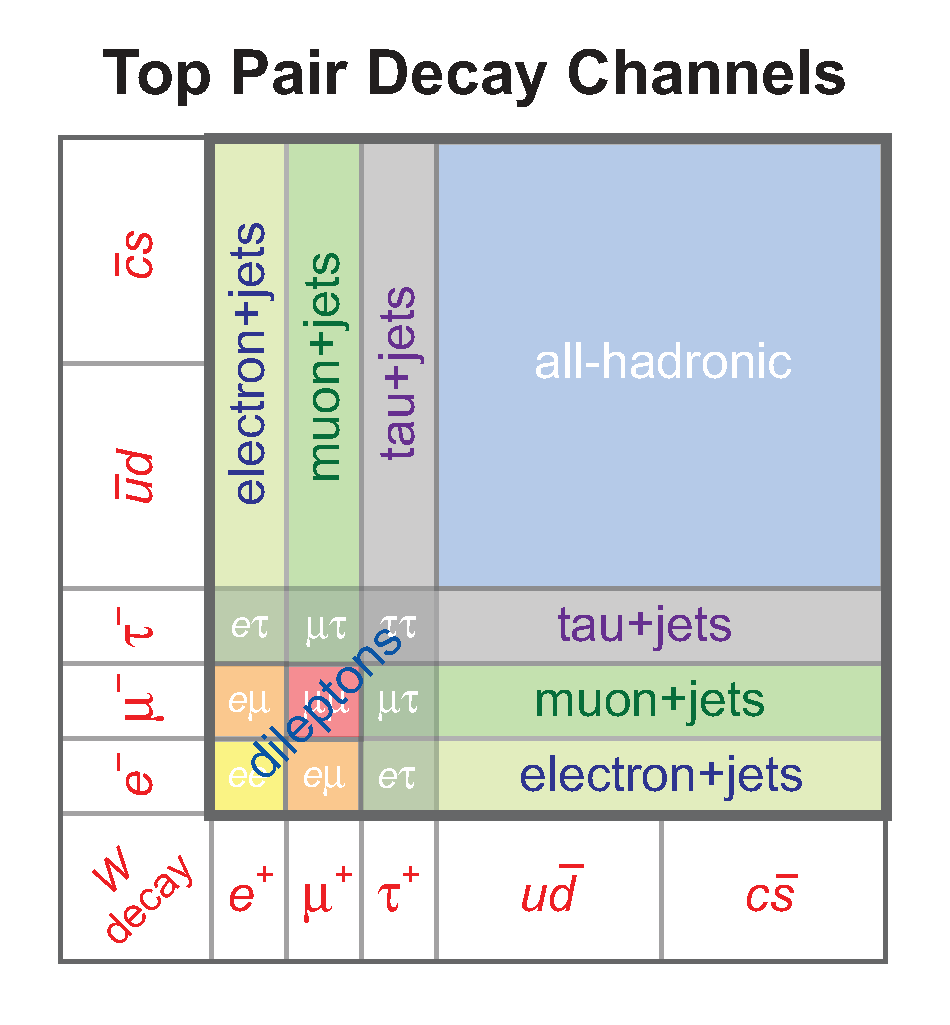
\includegraphics[width=0.5\textwidth]{Chapters/02_Theory/Images/top_pair_decay_channels.eps}\hfill
     \caption{Relative branching ratios of the \ttbar system}
     \label{fig:ttbar_branching_ratios}
\end{figure}

The signal event for this analysis is the semi-leptonic channel of the \ttbar decay, also referred to as
the lepton+jets channel, where the lepton is either an electron or a muon. These channels have a branching
ratio of apprimxately 14.2\% and 14.4\% respectively \cite{Agashe:2014kda}.

\subsection{Single Top background}
\label{ss:single_top}
Single top production is one of the backgrounds considered in this analysis, and can occur via the
electroweak interaction in one of three channels: s-channel or t-channel which involve the exchange of a
virtual \W boson, or tW-channel which involves the associated production of a \W boson and a \tquark. TODO:
INCLUDE FEYNMANN DIAGRAMS? %TODO: INCLUDE FEYNMANN DIAGRAMS?
Although semi-leptonic \ttbar decays have more jets in the final state than these single top production
modes, initial state radiation and final state radiation, where low energy gluons and quarks are produced
before and after the interaction that produces the single \t quark, can increase the numbers of jets in
single top events. This can lead to such events having a similar signature to \ttbar events, and providing a
non-negligble background.

\subsection{W/Z+jets background}
\label{ss:w_z_plus_jets}
\WpJets events present a significant background to semi-leptonic \ttbar analyses. This background
consists of events in which a real \W boson is produced together with additional jets. Events in which these
\W bosons decay leptonically, can provide a similar event signature after reconstruction to that of a
semi-leptonic \ttbar decay. However, in general, these processes can be removed from the signal selection
because the final decay products in \WpJets events have lower energies than those from semi-leptonic \ttbar
decays, since the top quark has a high mass. Another characteristic of \WpJets events is that the jets are
more likely to be light quark jets and therefore less likely to be the necessary \bjet s from \ttbar events.
Thus, \WpJets events can be separated from the \ttbar signal by using jet multiplicity, jet \pt and \bjet
multiplicity.

Similarly, \ZpJets events can mimic \ttbar events where the leptonic decay of \Z bosons to a lepton and an
anti-lepton takes place. This background can be distinguished and removed from semi-leptonic \ttbar decays by
vetoing on a second lepton and imposing jet multiplicity requirements. Misidentification and misreconstruction
of these leptons as jets, however, such events could appear to be \ttbar events and pass the signal selection,
although this contamination would be small. TODO:FEYNMANN DIAGRAM OF W \& Z PRODUCTION.
% TODO: FEYNMANN DIAGRAM OF W & Z + JETS EVENTS

\subsection{QCD background}
\label{ss:qcd}
The multi-jet background from QCD events is also a significant background to this semi-leptonic \ttbar
analysis. Gluon-gluon fusion, quark-antiquark annihilation can produce energetic jets (as shown in FEYNMANN
DIAGRAMS (TODO)).%TODO Although these processes have only two jets in their final state, higher order
processes, including initial state radiation and final state radiation, can also produce additional jets,
leading to potential mimicking of the semi-leptonic \ttbar signal. The leptons required for this to happen can
come from jets which are misreconstructed and misidentified as leptons, or real leptons in heavy flavour (\b
and \c flavour) jets. Unfortunately the cross section of these processes is much higher (by several orders of
magnitude) than the signal cross section. Although the lepton (either fake or real) is rarely one that passes
selection, the much higher QCD cross section means that its contribution as a background is significant.
% TODO: READ LUKE'S THESIS FOR WAYS IN WHICH JETS CAN FAKE AN ELECTRON OR A MUON

In the muon+jets channel, only highly energetic jets (\pt $> 500\GeV$) are capable of ``punching through''
from the calorimeters to leave tracks in the muon chambers. Such events can be removed by isolation (since it
deposits significant amounts of energy in the calorimeters) requirements. Events with real electrons and muons
from heavy quark jets can be identified by the track quality requirements in the selection since they would
not begin from the primary vertex and so would have a distrinct track signature compared to prompt leptons.

On the other hand, the electron channel poses a more problematic QCD background, due mainly to the conversion
of photons, whether produced at the interaction point or through subsequent decays and radiation, into
electrons and positrons. The identification and removal of such events is described in
Section~\ref{ss:electron_reconstruction}. However, the large uncertainty in the cross section of QCD events,
large contamination from higher order processes with additional jets in the signal region of this analysis and
the difficulty in Monte Carlo modelling of such contributions lead to significant disagreements in the numbers
of events passing the signal selection in data and in simulation. Therefore, the QCD background is modelled
using a data driven method.

The QCD background is difficult to model precisely because of large uncertainties on the cross sections and
the significant higher contributions which can easily be mismodelled, leading to incorrect event kinematics
and selection biases. Hence, the QCD background shape is modelled using a data driven method, decribed in
Section~\ref{ss:background_selection} and then normalised to the number of events passing the selection
process in Monte Carlo.


\subsection{tau leptons in semi-leptonic ttbar decays}
\label{ss:taus_in_semi-leptonic_decays}
 TODO: INSERT FEYNMANN
DIAGRAM OF TAU EVENTS %TODO: INSERT FEYNMANN DIAGRAMS FOR TAU DECAYS.

\section{Monte Carlo Simulation}
\label{s:monte_carlo_simulation}

Monte Carlo event simulation is used to simulate the aforementioned signal and background processes, and to
compare the theoretical knowledge of the Standard Model incorporated therein with real data. Differences
between simulation and data would then indicate the presence of new physics processes which are not present in
the theoretical assumptions made in the Standard Model, or perhaps that the simulation process is sub-optimal.
Different event generators exist, and samples produced by the \MADGRAPH, \PYTHIA, \POWHEG and \HERWIG
generators are used in this analysis.

Different generators have characteristics which optimise them for different aspects of the production chain:
the initial hard process scattering of the partons in the hadrons (protons), decay showers of the resulting
partons, subsequent decays of resulting hadrons and hadronisation of resulting partons, and the underlying
event (the parton showers produced from soft scattering between the remaining contents of the colliding
protons). 

\subsection{MadGraph}
\label{ss:madgraph}
\MADGRAPH \cite{madgraph5}, a matrix element generator, works by taking into account every potential Feynman
diagram for a given process and subsequently calculating the matrix elements for said diagrams over all phase
space. The cross section of the process and various subprocesses and the structure and contents of the event
(such as the partons present and their kinematics) are thus produced. %Also spin correlations. Also tau
% lepton decays
Proton fragmentation and subsequent hadronisation are simulated using the \PYTHIA generator, as explained in
Section~\ref{ss:pythia}. The parton showers are then matched with the matrix element partons via the MLM
method ~\cite{mlm}. This method ensures that parton showers with a highly energetic jet are not double
counted.

Matching is then carried out between parton showers in the hadronisation and the partons from the
matrix element calculations. The matching is carried out by satisfying distance requirements in $\eta$ and
$\phi$ between the parton and parton shower. Only if the parton has a transverse energy above a certain
threshold, is it considered for this matching, and if an event contains either too few or too many matching jets, it is
discarded. The matching threshold is process dependent as follows:
\begin{itemize}
  \item \ttbar: 20\GeV
  \item \WpJets: 10\GeV
  \item \ZpJets: 10\GeV
\end{itemize}

\subsection{MCatNLO}
\label{ss:mcatnlo}
The \MCATNLO \cite{mcatnlo_Frixione1, mcatnlo_Frixione2} generator is a next-to-leading-order generator. These
aditional corrections provide more accurate simulations of physics processes in comparison to leading-order
generators by including additional partons from the initial hard process in the final state of the event.

\subsection{PYTHIA}
\label{ss:pythia}
\PYTHIA \cite{pythia8} then simulates the proton fragmentation, the subsequent hadronisation of the
resulting quarks and gluons resulting from the hard interaction and the underlying event. \PYTHIA is
considered to be particuarly good at multi-particle simulation, modelling fragmentation and hadronisation, and
matching parton showers. Therefore, \PYTHIA carries out these steps after the initial partons are provided
by other generators in most simulated samples, if it is not already used for the whole production chain (as is
common in QCD multijet simulations).

\subsection{POWHEG}
\label{ss:powheg}
One problem with the \MCATNLO generator is that some events are given negative weights when matching
the next-to-leading-order QCD multijet calculations to parton showers.  The Positive Weight Hardest Emission
Generator, \POWHEG \cite{powheg_Frixione, powheg_Nason, powheg_Alioli}, is another next-to-leading-order
generator which generates the hardest processes in the event first, which avoids double counting of
softer radiation produced later in the chain, which is the cause of negative event weights.

%\subsection{HERWIG}
%\label{ss:herwig}
%\HERWIG \cite{herwig}
%TODO:HERWIG

\section{Theoretical Systematics}
\label{s:Theoretical Systematics}
\subsection{Factorisation \& Matching Threshold}
\label{ss:factorisation_and_matching_threshold}
Systematic uncertainties are present in the choice of the threshold transverse energy above which matching of
matrix element partons to parton showers is carried out. Simulated samples, in which the threshold is
increased and decreased by a factor of 2, are used to estimate the affect of this uncertainty on this
analysis:

\begin{itemize}
  \item \ttbar
  \begin{itemize}
    \item + variation: 40\GeV
    \item - variation: 10\GeV
  \end{itemize}
  
  \item \WpJets
  \begin{itemize}
    \item + variation: 20\GeV
    \item - variation: 5\GeV
  \end{itemize}

  \item \ZpJets
  \begin{itemize}
    \item + variation: 20\GeV
    \item - variation: 5\GeV
    \item \end{itemize}
\end{itemize}

Similarly, the factorisation scale at which $\alpha_{S}$ is varied up and down from the nominal value of
$Q^{2} = m^{2} + \Sigma p_{T}^{2}$ by a factor of 2 to produce simulation samples to evaluate the sytematic
uncertainty resulting from this. The uncertainty resulting from these variations are evaluated in both \ttbar
and \W/\ZpJets processes.
% TODO SMALL TABLE OF 0.5x and 2x variations?

\subsection{Detector Simulation (GEANT)}
\label{ss:detector_simulation}
Following creation of the physics processes in proton-proton collisions, the simulated events are then put
through a detector simulation to evaluate the interation of the detector with the products of collisions. The
Geometry and Tracking 4 (\GEANTfour) package is used for this purpose, which generally simulates what happens
to particles as they travel through the geometry of the detector, including simulation of the detector
components and materials and the interaction of particles with the detector such as particle tracks and energy
deposits.